\chapter{Chatbot}

El objetivo del bot es la recaudación de datos de usuarios mediante el uso de un agente conversacional como alternativa al tradicional cuestionario de preguntas. Para que al usuario le sea atractivo responder este tipo de cuestionarios que usualmente suelen ser un poco monótonos, he implementado una parte de interacción básica. Leyendo varias fuentes y opiniones de usuarios acerca de su experiencia con chatbots, 
 en \textit{(\cite{wellbeingchabot})} llegan a la conclusión de que a las personas entrevistadas les es mucho mas fácil poder abrirse y contestar preguntas acerca de su salud con un chatbot con el que pudieran conversar sabiendo que no hay lugar a ninguna crítica ni prejuicio por su parte, además de ser una experiencia calificada como más entretenida y divertida que realizar un cuestionario. Partiendo de esta base y con esa idea se ha desarrollado este proyecto. 

El agente conversacional se encuentra formado por 3 módulos diferenciados: Módulo de bienvenida y registro de usuario, módulo conversacional y cuestionario

\section{Módulo de bienvenida y registro}

La libreria \textit{python-telegram-bot} es la herramienta con la que vamos a interactuar con la API de Telegram. La librería emerge como una herramienta indispensable en este ámbito, proporcionando a los desarrolladores un marco completo para construir, desplegar y gestionar bots de Telegram sin esfuerzo.

Esta nos va a permitir diferentes posibilidades a la hora de crear nuestro bot como son la gestión de actualizaciones para controlar diferentes tipos de entradas de manera eficiente, envío de mensajes de texto y contenido multimendia, teclados y botones, comandos personalizados, respuestas interactivas, middleware y filtros. Todo lo relacionado a la descripción de estas operaciones se encuentra especificado en la documentación oficial \textit{(\cite{pythontelegrambot})}.

Este primer módulo tiene como objetivo la presentación de nuestro bot con el usuario y su registro en nuestra base de datos. \vspace{0.3cm}

Este módulo contiene una función que es la primera que se ejecuta cuando cualquier persona empieza una conversación. Se activa con el comando \textit{/start} que se envía mecánicamente y es el único comando necesario para la conversación. Cuando este evento se detecta se realiza una llamada a la función la cual muestra un mensaje de bienvenida al usuario presentando los temas a tratar. Gracias a la librería usada podemos obtener los datos que el usuario posea en su Telegram personal (como el nombre, nombre de usuario, apellidos, email, id).\vspace{0.3cm}

\begin{lstlisting}[language=Python]
    suscriber, created = Suscriber.objects.get_or_create(
        chatid = chat_id,
        name=name,
        surname=surname,
        username=username,
    )
\end{lstlisting}

 La función de Django \textit{get\_or\_create()} nos permite filtrar una serie de datos introducidos dentro de una tabla en la base de datos. En caso de ningún registro coincida exactamente con todos los datos, crea una nueva instancia con los parámentros pasados. De esta forma se registran los usuarios. Para asegurarnos de la concurrencia de nuestro programa, he creado una atributo en usuario llamado chatid que almacena el id propio del chat. Esto se hace con la intención de no declarar variables globales dentro del código ya que si hubiera varias personas hablando al mismo tiempo habría problemas de concurrencia. Por eso cada consulta y cada mensaje es específico para cada uno intentando operar siempre desde la base de datos lo que además influye positivamente en la eficiencia ya que las consultas y operaciones son más rápidas.\vspace{0.3cm}


\begin{figure}[!ht]
    \centering
    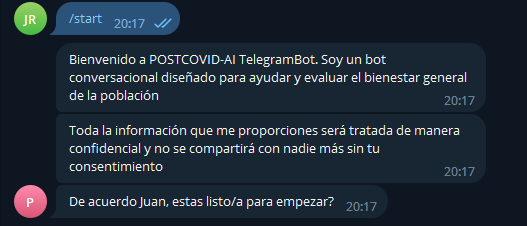
\includegraphics[width=1\textwidth]{imagenes/welcome.png}
    \caption{ Mensaje de bienvenida }
    \label{fig:enter-label}
\end{figure}\vspace{1cm}

Este es el mensaje de presentación del bot. Nos pone en contexto y nos habla sobre su propósito. Finalmente nos hace una pregunta y dependiendo de la respuesta del usuario nos redigirá a un módulo u otro. 

\section{Módulo conversacional}

Este módulo es una etapa intermedia, que funciona como una especie de sala de espera a que el usuario cuente con cuestionarios a responder. Dentro de él, se puede tener una conversación de lo más común y simple con el bot, con un apartado que muestra preguntas frecuentes en caso de que el usuario tenga cualquier tipo de duda. 

El usuario puede entrar dentro de este módulo de diferentes maneras. Una de ellas es respondiendo de forma negativa en la pregunta anterior. Dentro de este módulo hay unas palabaras, frases o expresiones previamente definidas por las cuales el bot responde en función de lo que escribas. Cabe destacar que no se utiliza modelos de lenguaje como GPT para generar respuestas mas elaboradas. GPT es un modelo que utiliza algoritmos avanzados de procesamiento de lenguaje natural para generar respuestas a preguntas y comentarios de los usuarios en tiempo real \textit{(\cite{gpt2020})}. En nuestro caso esa no es la finalidad de nuestro bot, como dije el propósito principal es la recogida de datos, con la funcionalidad añadida de que el usuario pueda tener una conversación escueta con el bot para que esta recogida se realice de la forma más humanamente posible, pero esta quedando siempre en el segundo plano. 

Este módulo se ejecuta de forma recursiva cada vez que el usuario escribe un mensaje en el chat. Funciona de la siguiente manera:\vspace{0.3cm}

\textbf{1. Recogida del mensaje: }Cuando el usuario manda cualquier tipo de mensaje el bot lo recibe como texto de entrada y lo almacena.\vspace{0.3cm}

\textbf{2. Procesamiento: }Este proceso implica limpiar y normalizar el texto introducido, convirtiéndolo a minúsculas y reduciendo las palabras a su forma base. \vspace{0.3cm}

\textbf{3. Análisis: }Conlleva la identificación del contexto del mensaje con el propósito de extraer información relevante o identificar intenciones. 

Esta identificación se hace dentro del archivo \textit{replyMessages.py} situado dentro de la carpeta /chatbot. En el podemos encontrar diferentes listas como estas.

\begin{lstlisting}[language=Python]
#HELLO AND GOOD BYE
greetings = ['hola', 'hello', 'buenos dias', 'buenas tardes', 'buenas', 'saludos', 'hi', 'good']
farewell = ['adios', 'bye', 'good bye', 'hasta luego', 'nos vemos', 'hasta pronto', 'buenas noches', 'que tengas un buen dia', 'hasta la proxima','que vaya bien']

\end{lstlisting}

Este es un ejemplo de lista para establecer el contexto de saludo y despedida. Estas listas definen una serie de palabras y expresiones concretas que cualquier persona hispanohablante utilizaría si quisiera referirse o hablar sobre un tema. Si cualquier palabra dentro de la respuesta del usuario se encuentra contenida en esta lista el bot identifica la intención del mensaje y le asociará un contexto.\vspace{0.3cm}

\textbf{4. Generación de respuesta: }Una vez encontrado el contexto del mensaje debemos buscar una respuesta digna que se adecue al tema tratado. Para ello dentro de este mismo archivo mencionado encontramos varios diccionarios. Estos contienen las respuestas que el bot debe proporcionar para cada contexto. Por ejemplo:

\begin{lstlisting}[language=Python]
    'greetings':{
        '0': 'Hola!¿Puedo ayudarte en algo?',
        '1': 'Muy buenas!¿Necesitas ayuda?',
        '2': 'Hola!¿Como puedo asistirte hoy?'
    },
    'farewell':{
        '0': '¡Adios!.¡Que tengas un buen dia!',
        '1': 'Hasta luego!.¡Espero verte de nuevo pronto!',
        '2': 'Adios. !No dudes en volver!',
    },
\end{lstlisting}

Cuando declaramos el contexto de saludo como este ejemplo, vemos que hay una serie de mensajes. He intentado que haya un mínimo de unos tres mensajes por cada contexto para que la respuesta proporcionada por el bot no sea siempre igual e intentar que esta varie. \vspace{0.1cm}

A la hora de mostrarlo en el chat se hace con la función de debajo que envía el mensaje al usuario en concreto que lo ha escrito y selecciona una respuesta aleatoria dentro de las que el diccionario disponga.\vspace{0.3cm}

\begin{lstlisting}[language=Python]
context.bot.send_message(chat_id=user.id, text=messages['greetings'][str(random_var)])
\end{lstlisting}

Por último debemos tratar que pasaría si el bot no reconoce el mensaje del usuario, ya sea por hablar de un tema que el bot no tiene respuesta o por escribir mal una palabra o expresión. En este caso, en la etapa anterior de análisis el bot no podría clasificar la respuesta. Cuando esto sucede se muestra lo siguiente:\vspace{1cm}

\begin{figure}[!ht]
    \centering
    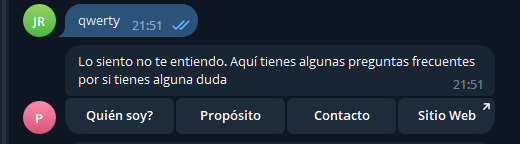
\includegraphics[width=1\textwidth]{imagenes/no_respuesta.png}
    \caption{ Mensaje no entendido }
    \label{fig:enter-label}
\end{figure}\vspace{0.3cm}

El mensaje contiene botones con algunas preguntas frecuentes que puedan ser de interés al usuario (como información sobre el bot, su propósito, sitio web y contacto del proyecto a que pertenece). Estos son los mensajes que mostraría si pulsas cada uno de los botones:\vspace{0.3cm}

\begin{figure}[!ht]
    \centering
    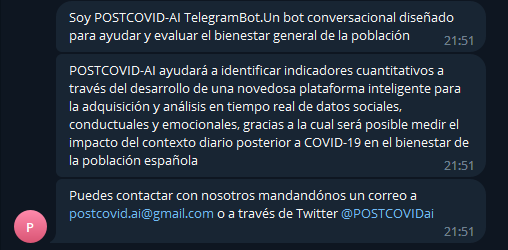
\includegraphics[width=1\textwidth]{imagenes/preguntas_frecuentes.png}
    \caption{ Preguntas Frecuentes }
    \label{fig:enter-label}
\end{figure}\vspace{0.3cm}

\subsection{Job pendiente del usuario}

Desde el primer momento que el usuario entra dentro de este módulo se crea un proceso recursivo dentro del mismo que se ejecuta cada 24 horas. Este proceso se inicia cada vez que el usuario cuente con preguntas pendientes por responder. Para comprobar esto, el bot cuenta con un método que recorre las respuestas del usuario y compara la fecha de cuando esa pregunta fue respondida con la fecha actual. Recordemos que los bloques tienen una frecuencia, hay algunos que deben hacerse todos los días y otros una vez por semana. Pues esta función comprueba si el resultado de la resta de esta fecha pasado a segundos es mayor que la frecuencia del bloque también en segundos, significa que ha pasado el tiempo de frecuencia de ese bloque por lo que se vuelve a encontrar activo en el sistema y el usuario contará con preguntas pendientes. 

Cuando este usuario tenga preguntas se inicializa lo que según la libreria de \textit{python-telegram-bot} se denomina como 'Job'. Este Job es un proceso que se ejecuta cada un tiempo determinado y que solo termina cuando sucede un evento concreto. 

\begin{lstlisting}[language=Python]
    def create_job(self, context):
        #Create a user's job
        context.job_queue.run_repeating(callback=self.job, interval=86400, first=0, context=self.suscriber.chatid, name=self.suscriber.chatid)
\end{lstlisting}

Esta es una forma de crear el Job y como vemos este se ejecuta cada 24 horas y básicamente lo que hace es mostrar el siguiente mensaje al usuario para avisarle de que tiene preguntas activas (si se cumple la condición de que las tenga) y puede pasar a responderlas.

\begin{figure}[!ht]
    \centering
    
\includegraphics[width=1\textwidth]{imagenes/mensaje_preguntasactivas.png}
    \caption{ Mensaje preguntas pendientes }
    \label{fig:enter-label}
\end{figure}\vspace{0.3cm}

Este proceso solo termina cuando el usuario empieza a responder el cuestionario de preguntas. Si no lo hace, cada 24 horas el bot enviará el mensaje de nuevo. 

\section{Módulo cuestionario}


Pasamos ahora al último módulo y más importante de nuestro bot. Este módulo sigue el ejemplo de un cuestionario de preguntas clásico en el que el bot te va haciendo una serie de preguntas y tu debes responder con una de las opciones posibles conforme al criterio de cada uno. 

Para entrar, el bot ya sea al principio o cuando contemos con preguntas pendientes nos hará la pregunta de si queremos comenzar el cuestionario. Solo entraremos en él cuando respondamos de forma afirmativa a esta pregunta. 

Una vez estemos dentro, el bot nos explicará de forma escueta como funciona y eligirá la primera pregunta. He aquí cuando entra en juego una de las funciones principales \textit{chooseQuestion(user)}.

Esta función lo que hace es recorrer los bloques de preguntas que se encuentra activos en el sistema ordenándolos por importancia. Comprueba las preguntas una a una dentro de cada bloque filtrando las respuestas para cada usuario y comprobando si ha sido respondida. En este punto tenemos dos posibilidades. Que el usuario sea nuevo y no ha realizado ningún cuestionario, por lo que la primera pregunta que compruebe será la devuelta ya que no hay ningún registro de respuestas por su parte. Y en caso contrario, que el usuario ya haya realizado varios cuestionarios. En este supuesto, se resolvería de la misma forma que el Job entiende cuando un usuario cuenta con preguntas pendientes, es decir, comparando las fechas de las respuestas con la fecha actual, restándola y si es mayor a la frecuencia del bloque, significa que esa pregunta se encuentra pendiente, si no pasaría a la siguiente. Además el método identifica la primera pregunta perteneciente a cada bloque, para que cuando esta se haga muestre cualquiera de los mensajes asociados al contexto de ese bloque de preguntas.

Para el cuestionario se ejecuta recursivamente la función \textit{handleanswer(update, context)} y solo termina cuando el usuario no cuente con preguntas pendientes. En cada iteracción hace una llamada a la función anterior, elije la pregunta a realizar al usuario y muestra el mensaje del contexto si es la primera pregunta del bloque. \vspace{0.3cm}

\begin{figure}[!ht]
    \centering
    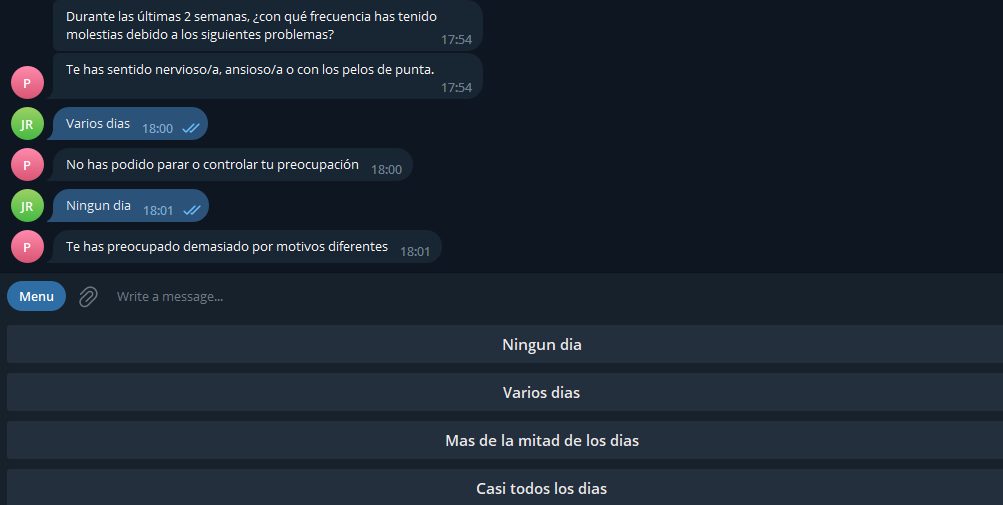
\includegraphics[width=1\textwidth]{imagenes/question.png}
    \caption{ Cuestionario }
    \label{fig:enter-label}
\end{figure}\vspace{0.3cm}

Ya sabemos que cada pregunta cuenta con posibles respuestas de forma independiente. Como podemos ver en la figura 4.5 el bot cuando hace la pregunta nos actualiza el teclado de Telegram y nos da la opción solo de contestar mediante botones que contienen las respuestas a la pregunta. Esto se hace de la siguente manera:

\begin{lstlisting}[language=Python]
#Function to get a custom keyboard in Telegram
def custom_keyboard(values):
    schema = [[str(value)] for value in values]
    return ReplyKeyboardMarkup(schema, one_time_keyboard=True, resize_keyboard=True)
\end{lstlisting}

El parámetro pasado contiene las respuestas a la pregunta y haciendo uso de la función \textit{ReplyKeyboardMarkup()} proporcionada por la libreria de Telegram creamos un teclado personalizado con los valores que deseemos. Solo podemos responder a la pregunta si el mensaje esta dentro de estas respuestas. Esto lo hice para asegurarnos que los datos obtenidos son correctos y reales, ya que si respondemos cualquier cosa que no tuviera nada que ver se guardaría como respuesta a la pregunta. Por lo que en cada iteracción de la función se comprueba si el mensaje proporcionado por el usuario es válido. En caso negativo, el bot no pasaría a la siguiente pregunta y volverá a realizarla de forma indefinida hasta que respondas de forma correcta. \vspace{0.3cm}

\begin{figure}[!ht]
    \centering
    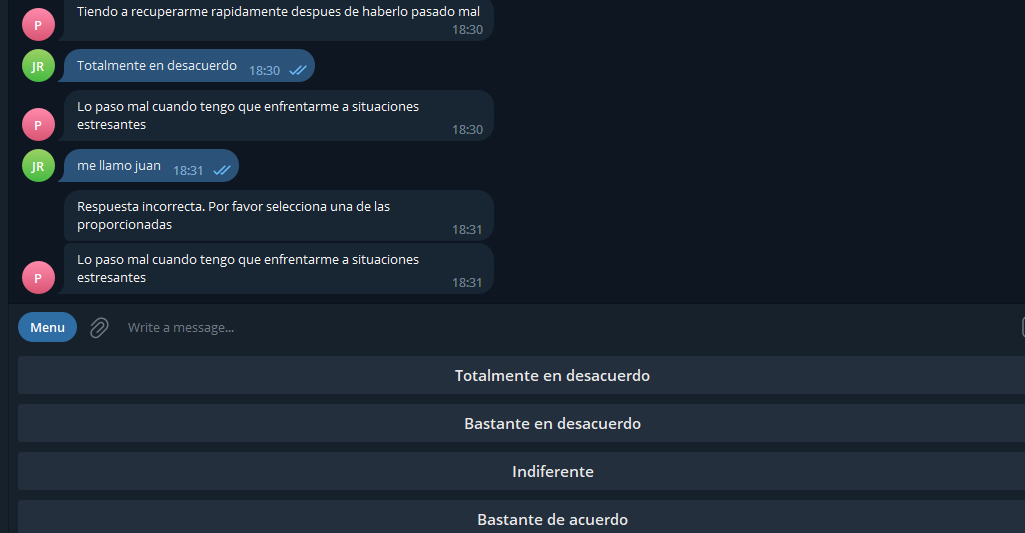
\includegraphics[width=1\textwidth]{imagenes/pregunta_incorrecta.png}
    \caption{ Respuesta incorrecta }
    \label{fig:enter-label}
\end{figure}\vspace{0.3cm}

Solo cuando esta sea correcta guardará la respuesta en la base de datos. La función finaliza cuando el usuario haya terminado de responder todas las preguntas y te redirigirá de forma automática al módulo conversacional creando un Job para el usuario que te avisará cuando cuentes de nuevo con preguntas pendientes. \vspace{1cm}


Recapitulando todo el proceso, cuando inicies una conversación con el bot, este te registrará en la base de datos como un nuevo usuario. Empezarás realizando el cuestionario de preguntas que se encuentre activo para tí en ese momento y cuando lo termines te llevará al módulo conversacional en el que puedes charlar con el bot. Cuando el sistema identifique que tienes preguntas pendientes te lo hará saber con un mensaje que se manda automáticamente cada 24 horas y que solo termina cuando las vuelvas a responder.